%=== CHAPTER FIVE (5) ===
%=== Discussion ===

\chapter{Result \& Discussion}
\begin{spacing}{1.5}
\setlength{\parskip}{0.3in}
\begin{figure}[h]
    \centering
    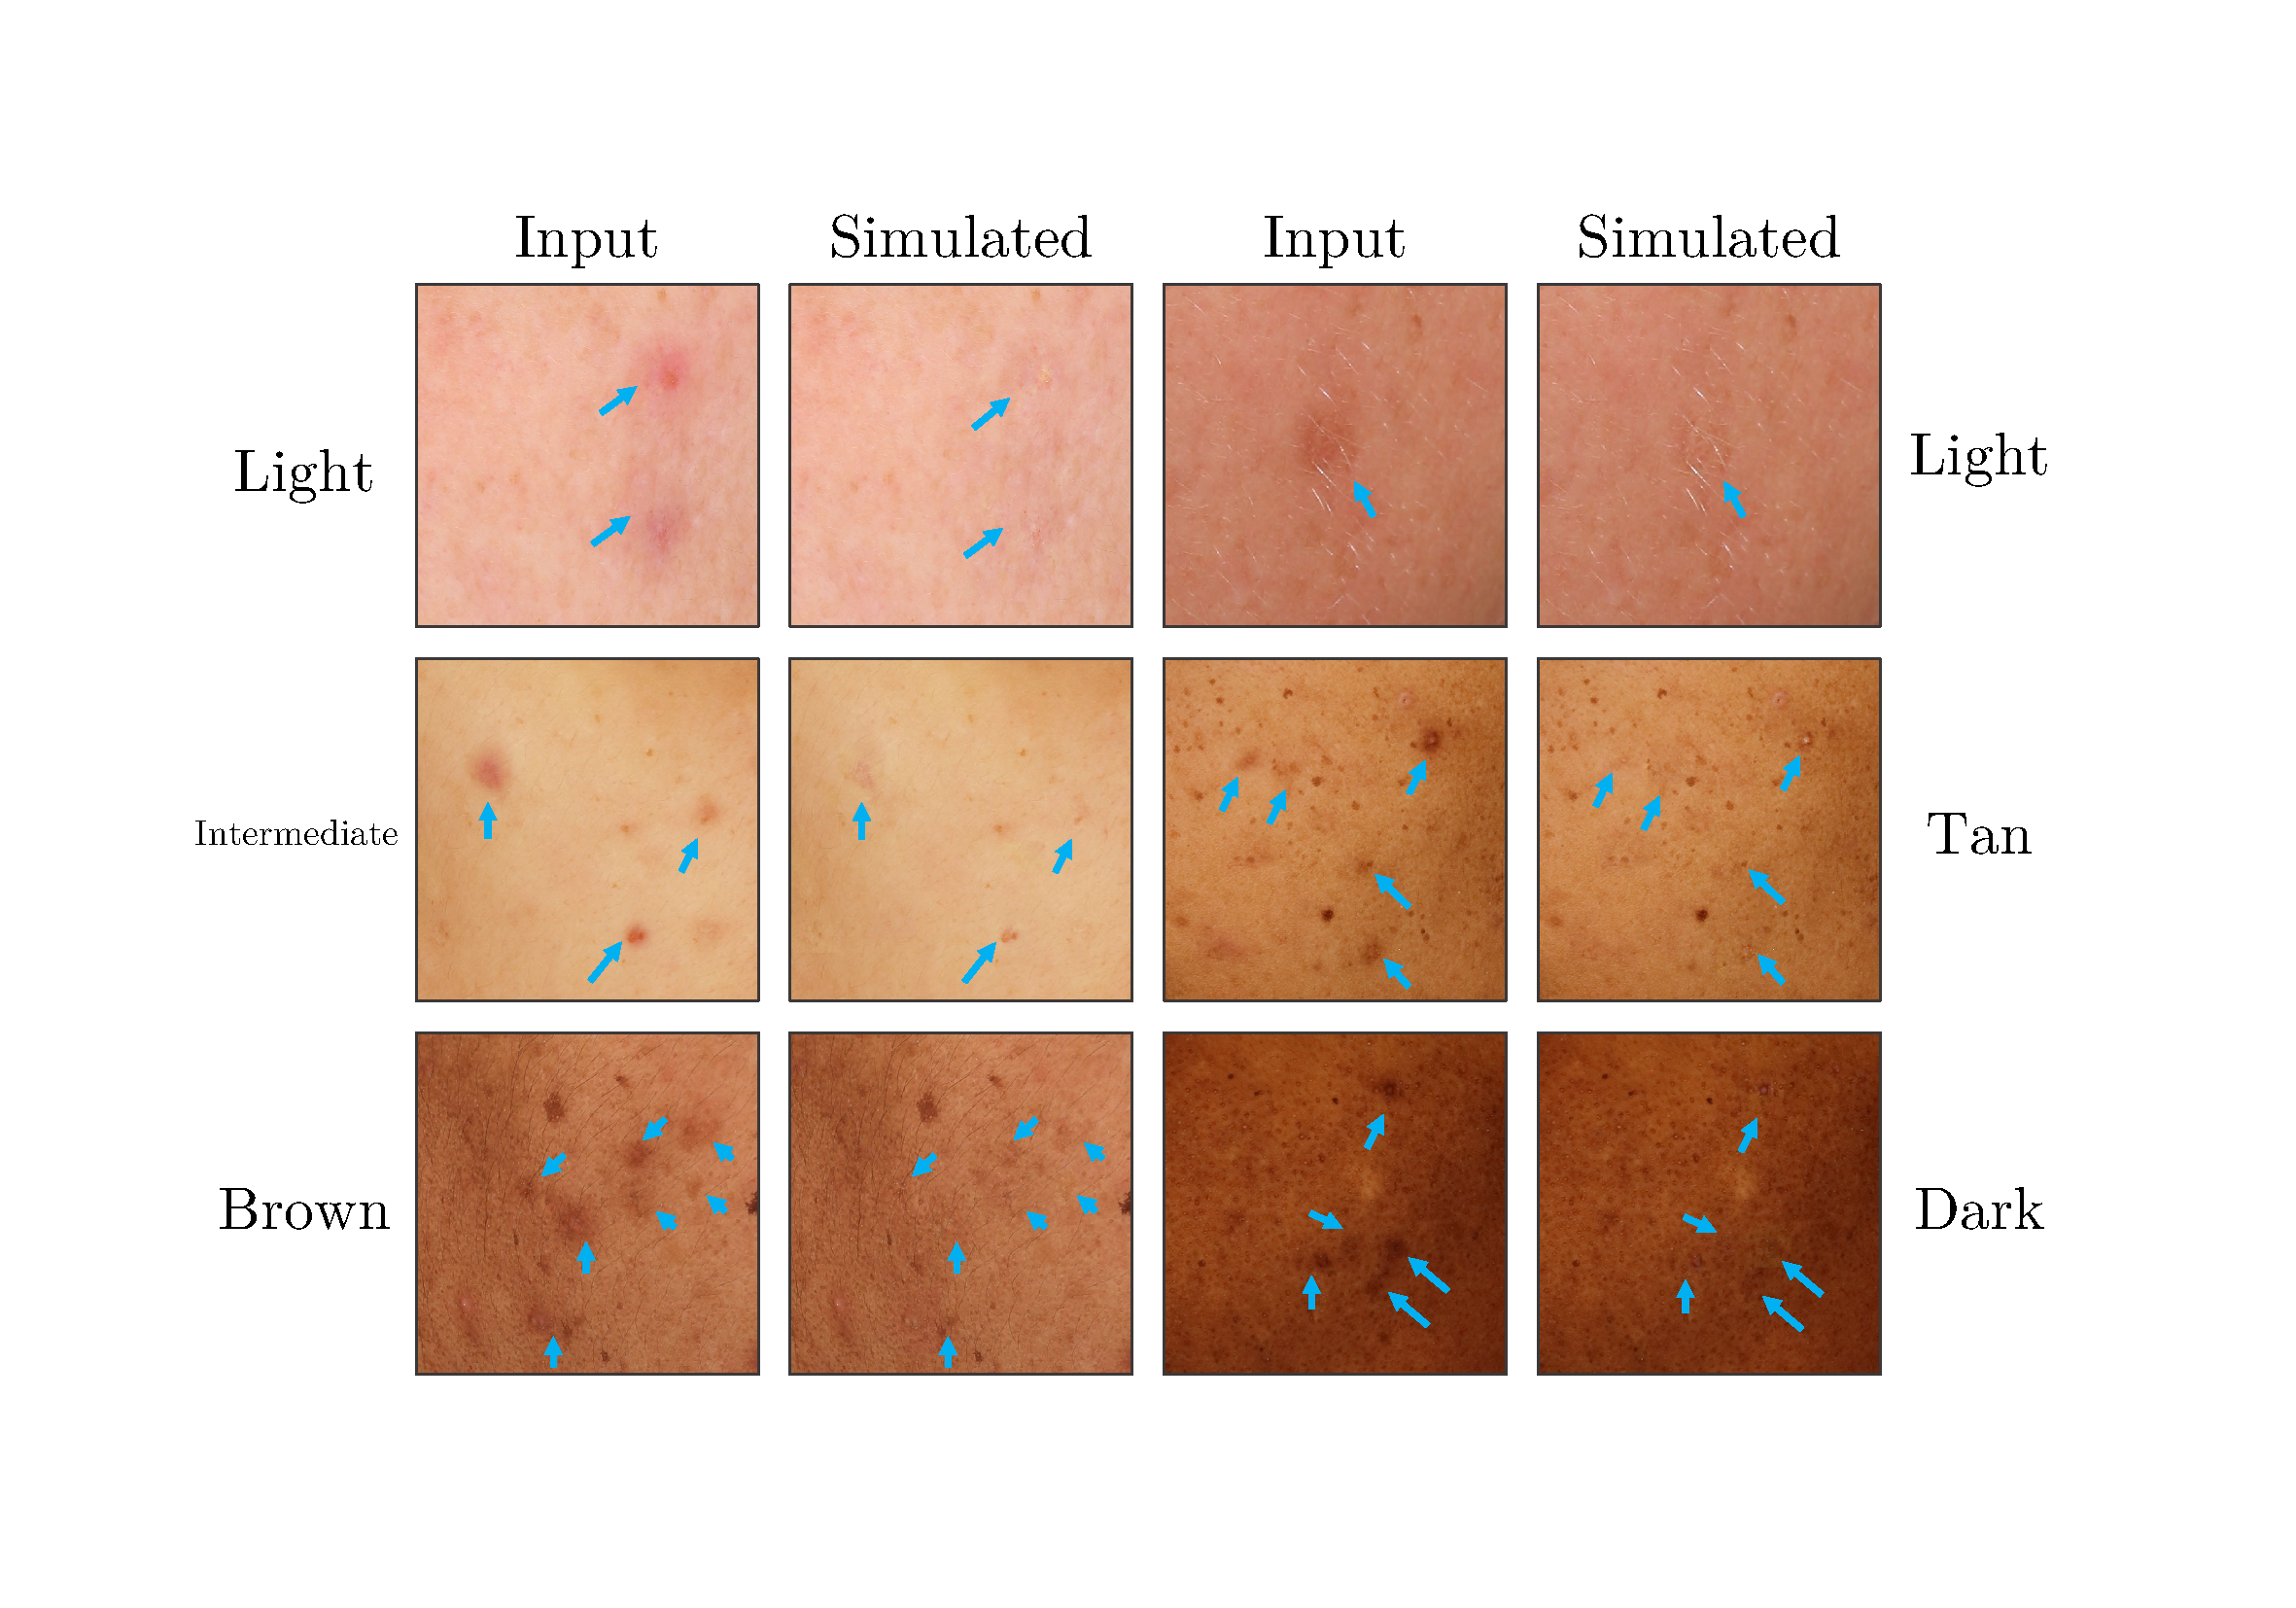
\includegraphics[width=\columnwidth]{Chapter5/img_comp6.pdf}
    \caption{Simulation under various skin tones with zoomed-in details. Blue Arrows are manually added to highlight blemishes of interest (acne or pigmentation). And the skin tone classification is labeled on the side of the figure. Note that the proposed method keeps skin details (e.g., hairs, texture) unaltered and can achieve realistic blemish removal under different skin tones.}
    \label{fig:sim1}
\end{figure}
The simulation quality and result are evaluated in terms of versatility, reality, and controllability. A detailed discussion of each aspect follows.
\section{Versatility}
Versatility is a key attribute of the proposed algorithm's ability to be generalized to various scenarios. By testing various patterns and degrees of pigmentation, acne, and other skin aberrations, the successful application of the proposed algorithm on multiple skin tones and different types of skin blemishes is demonstrated. Figure \ref{fig:sim1} clearly illustrates how the proposed algorithm accurately models the local chromophore enrichment of the skin, thus realizing genuine blemish change simulation. Particularly noteworthy is that the proposed method maintains the subtle textures of the skin unaltered, as fine hairs or pores shown in Figure \ref{fig:sim1}, further proving its high precision and usability.
% \begin{figure}[t]
%     \centering
%     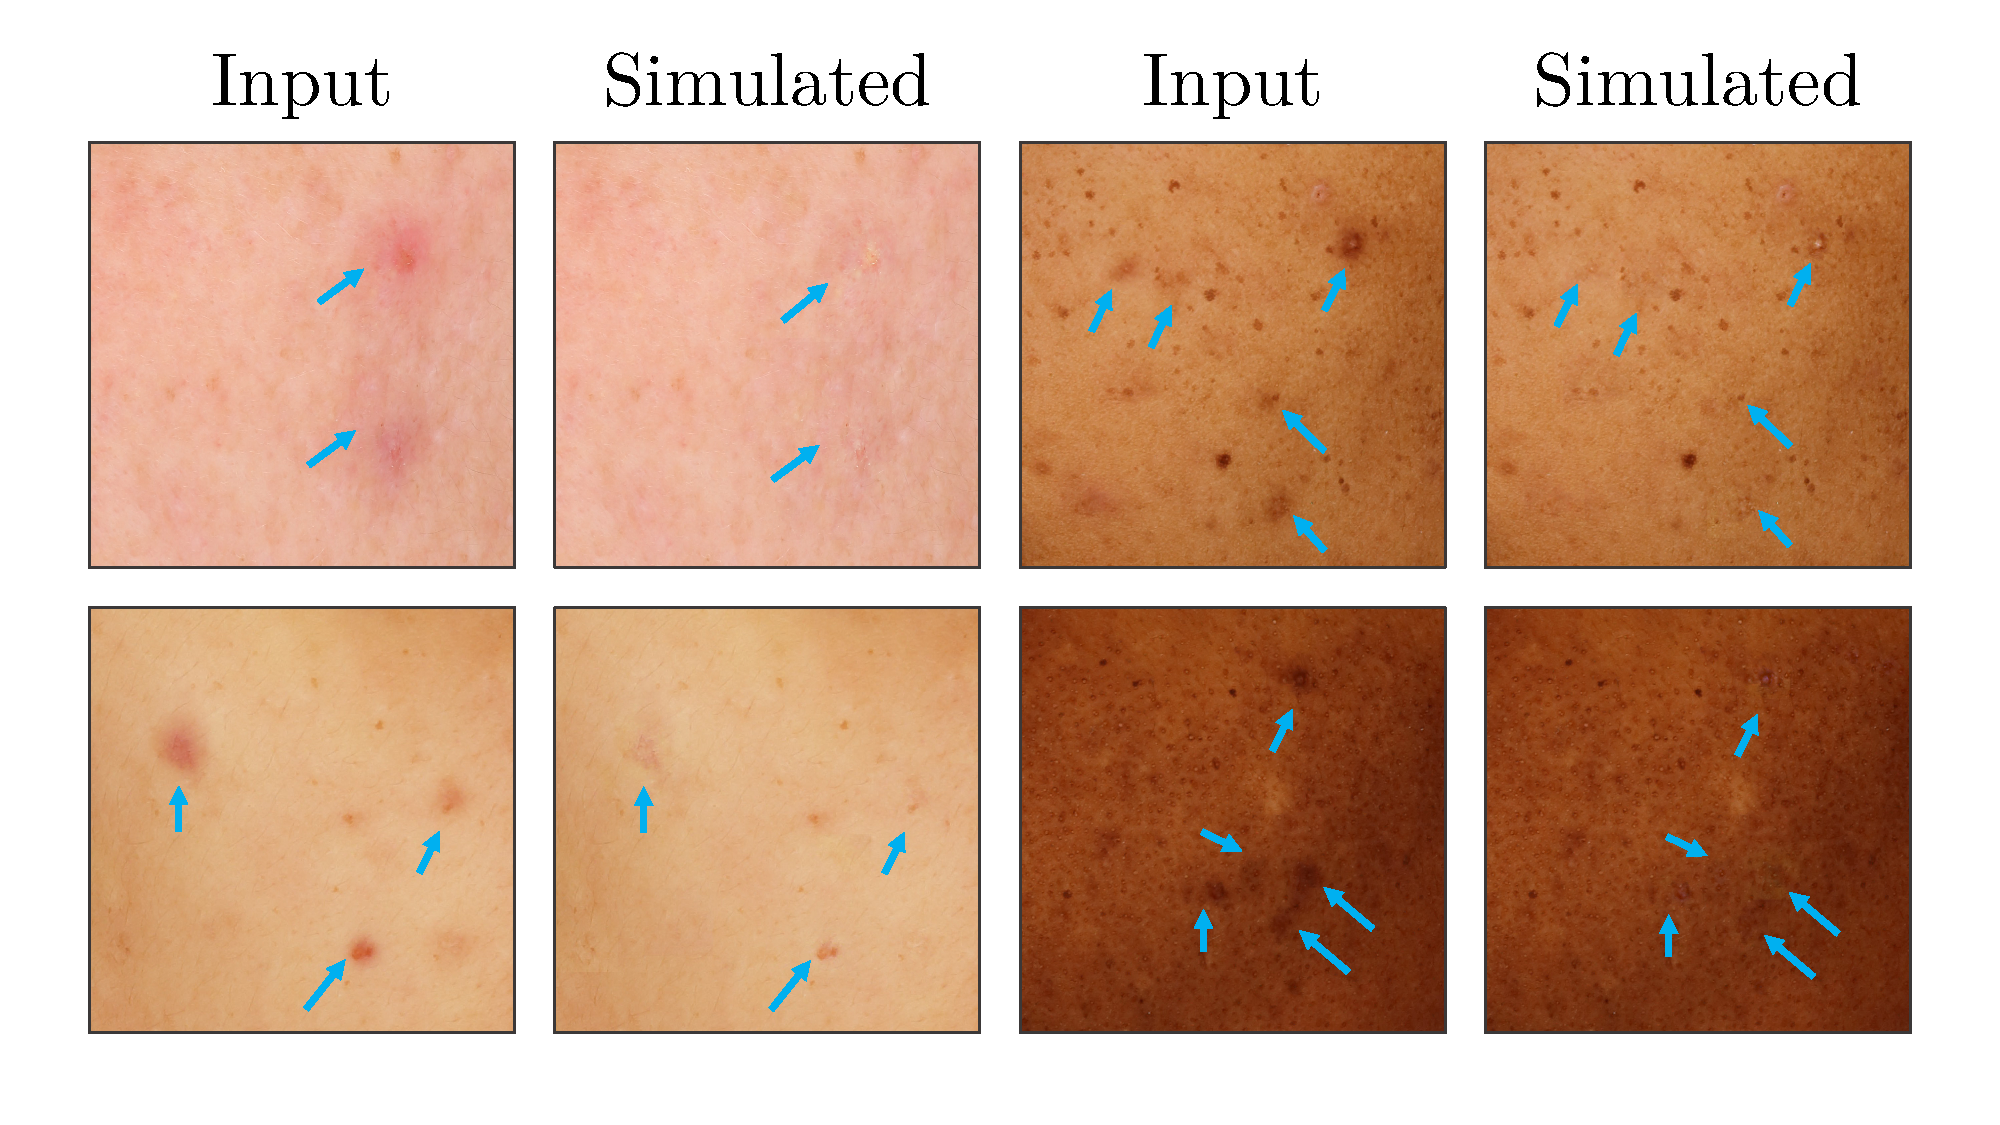
\includegraphics[width=\columnwidth]{Chapter5/img_comp4.pdf}
%     \caption{Simulation under various skin tones}
%     \label{fig:sim1}
% \end{figure}

\section{Reality}
\begin{figure}[t!]
    \centering
        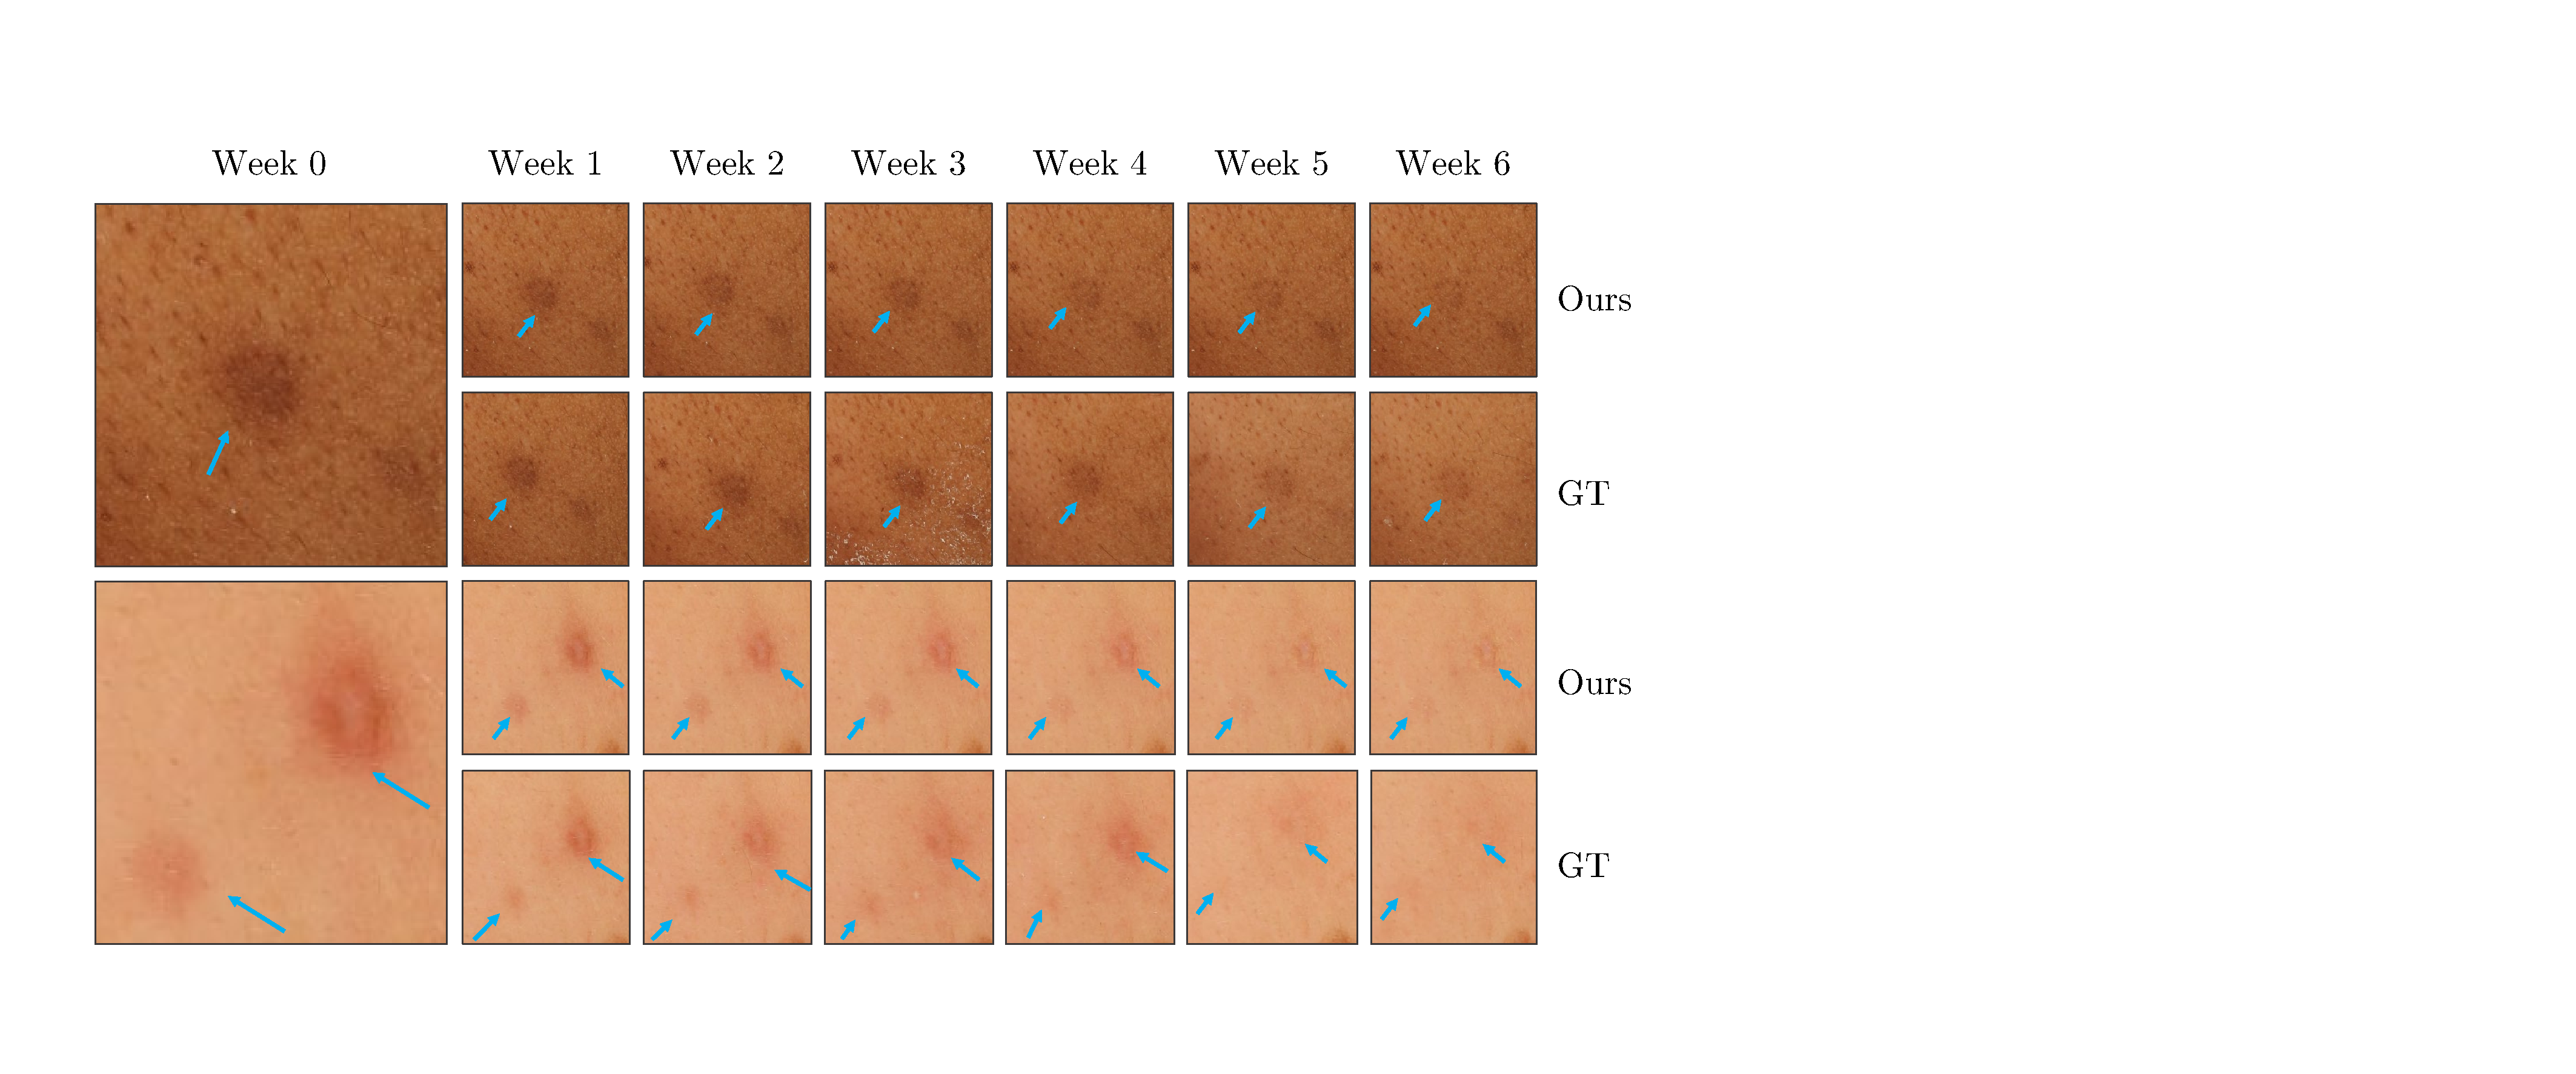
\includegraphics[width=\columnwidth]{Chapter5/forward3.pdf}
    \caption{The application of the proposed method to the simulation of the fading process of skin blemish is shown. Blue Arrows are manually added to highlight blemishes of interest (acne or pigmentation). In the simulation, images of \textit{Week 0} are input and the parameters of the obtained model are adjusted to simulate the change of the blemishes in the following weeks. Note that the proposed method applies to different skin tones and various types of blemishes.}
    \label{fig:forward}
\end{figure}
Exploration of reality evaluates the proposed algorithm's ability to simulate complex changes in real human skin conditions. Some skin blemish samples with long-term evolution patterns from the dataset are selected and simulated using the proposed algorithm. Figure \ref{fig:forward} shows one example, revealing the gradual fading of pigmentations over 7 weeks. The proposed algorithm successfully simulates the natural fading trajectory of the pigmentations, showing a natural change in color.

Fréchet Inception Distance (FID) scores for the simulated images and the ground-truth images are calculated to quantitatively measure the quality of algorithms for skin blemish editing. The results are displayed in Table \ref{tbl:fid} and the visual comparison is shown in Figure \ref{fig:baseline}.
\begin{figure}[t!]
    \centering
    \begin{subfigure}{\textwidth}
        \centering
        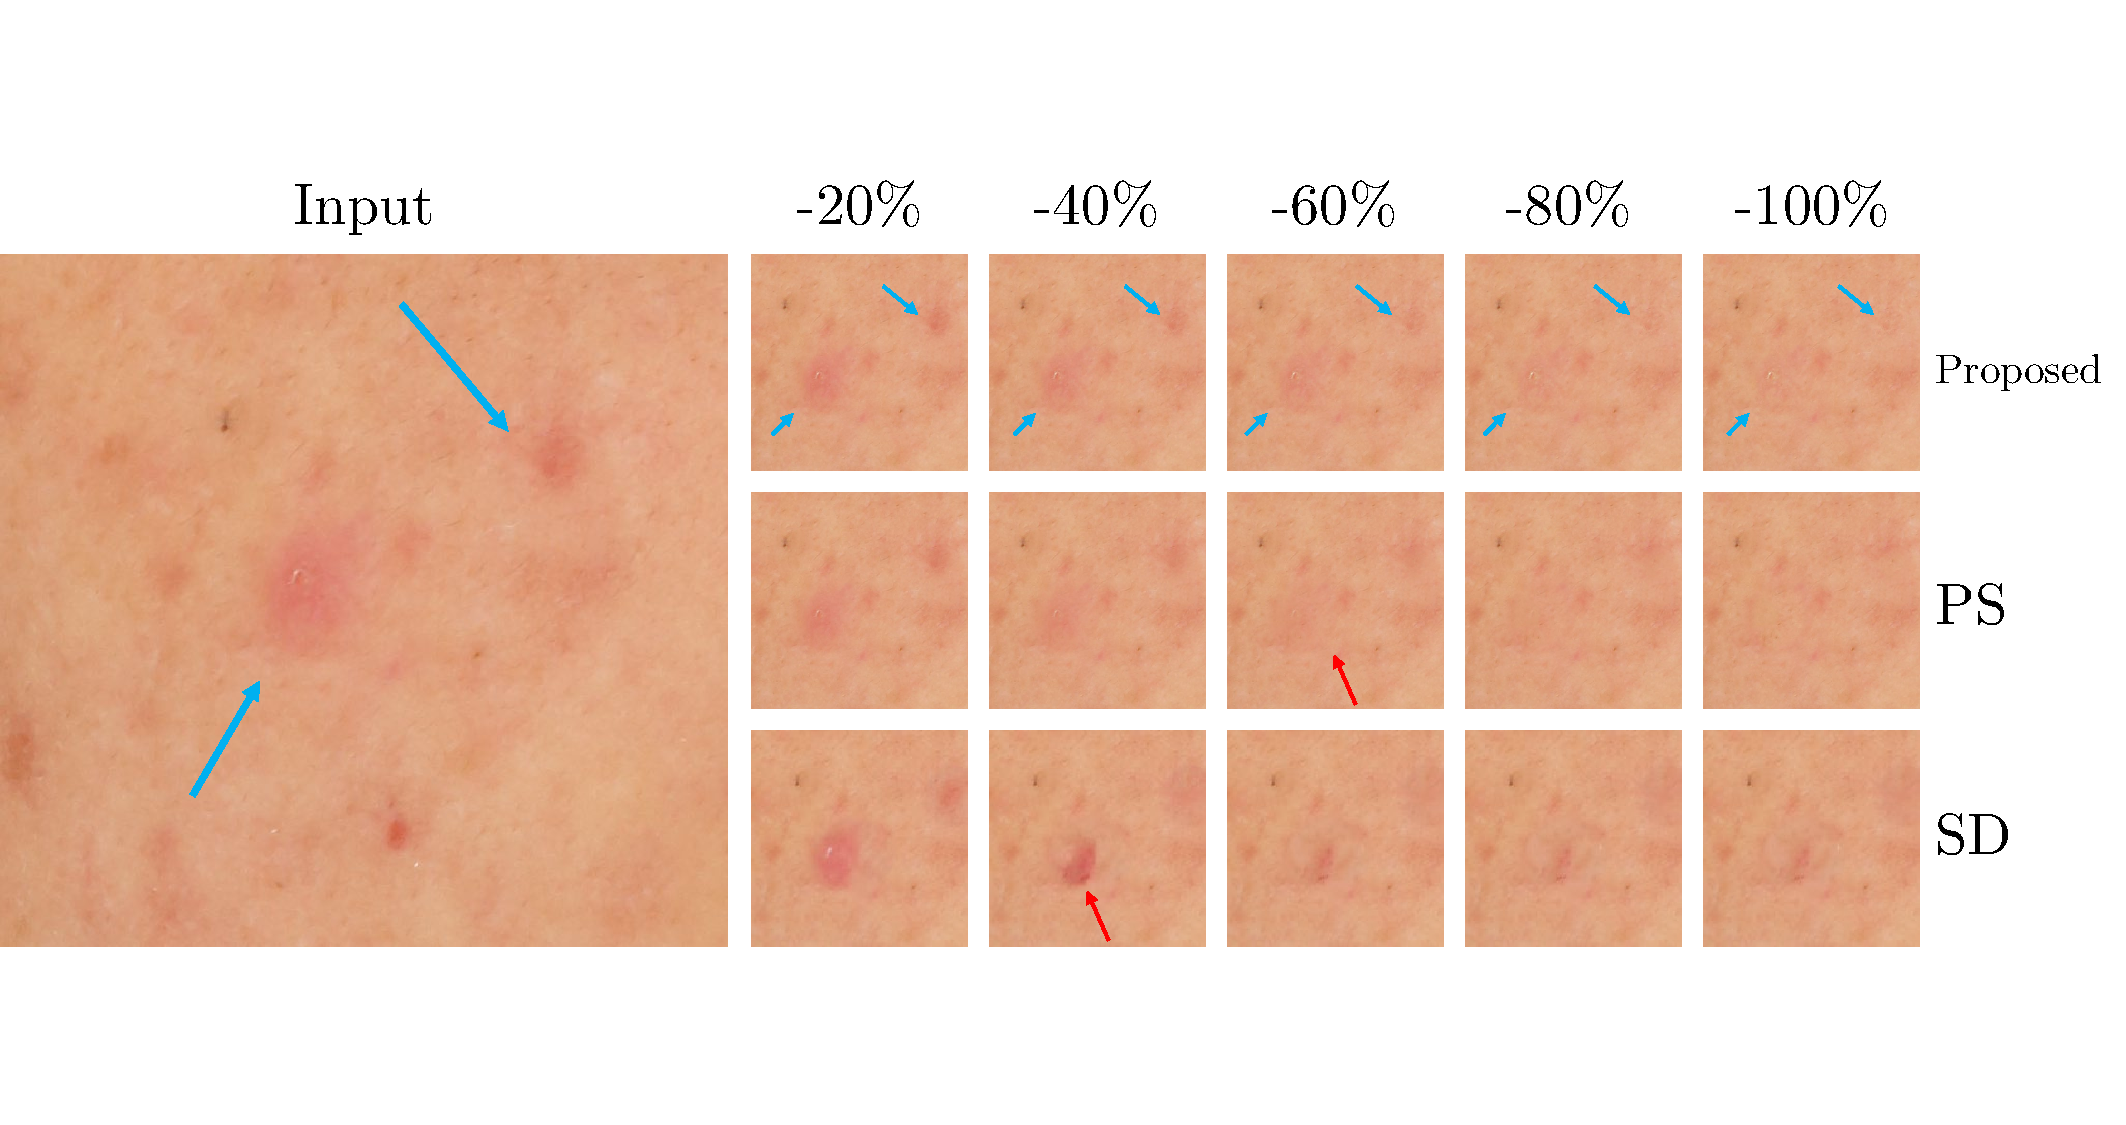
\includegraphics[width=\linewidth]{Chapter5/baseline/baseline41.pdf}
    \end{subfigure}
    \hfill
    \begin{subfigure}{\textwidth}
        \centering
        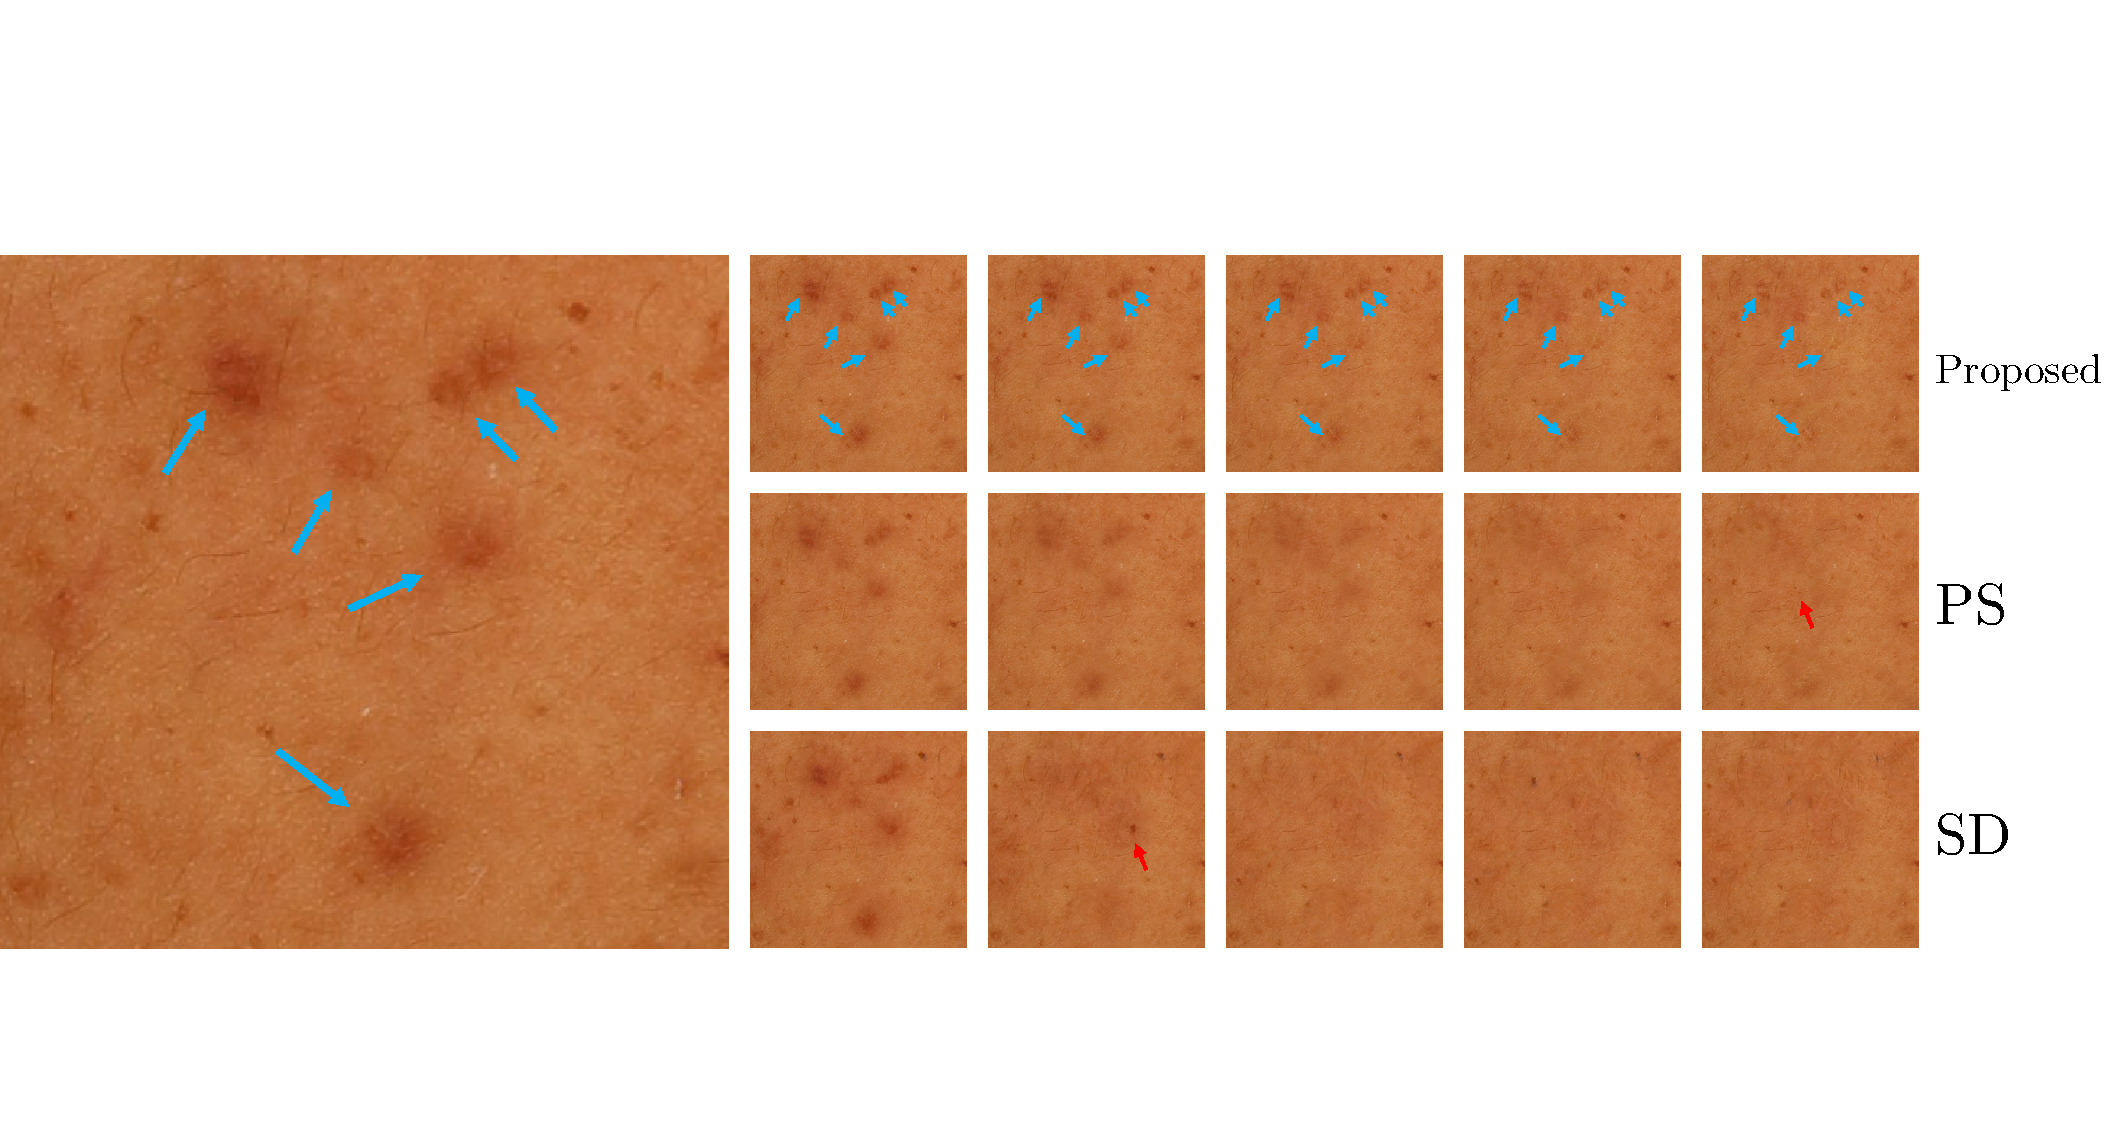
\includegraphics[width=\linewidth]{Chapter5/baseline/baseline42.pdf}
    \end{subfigure}
    \hfill
    \begin{subfigure}{\textwidth}
        \centering
        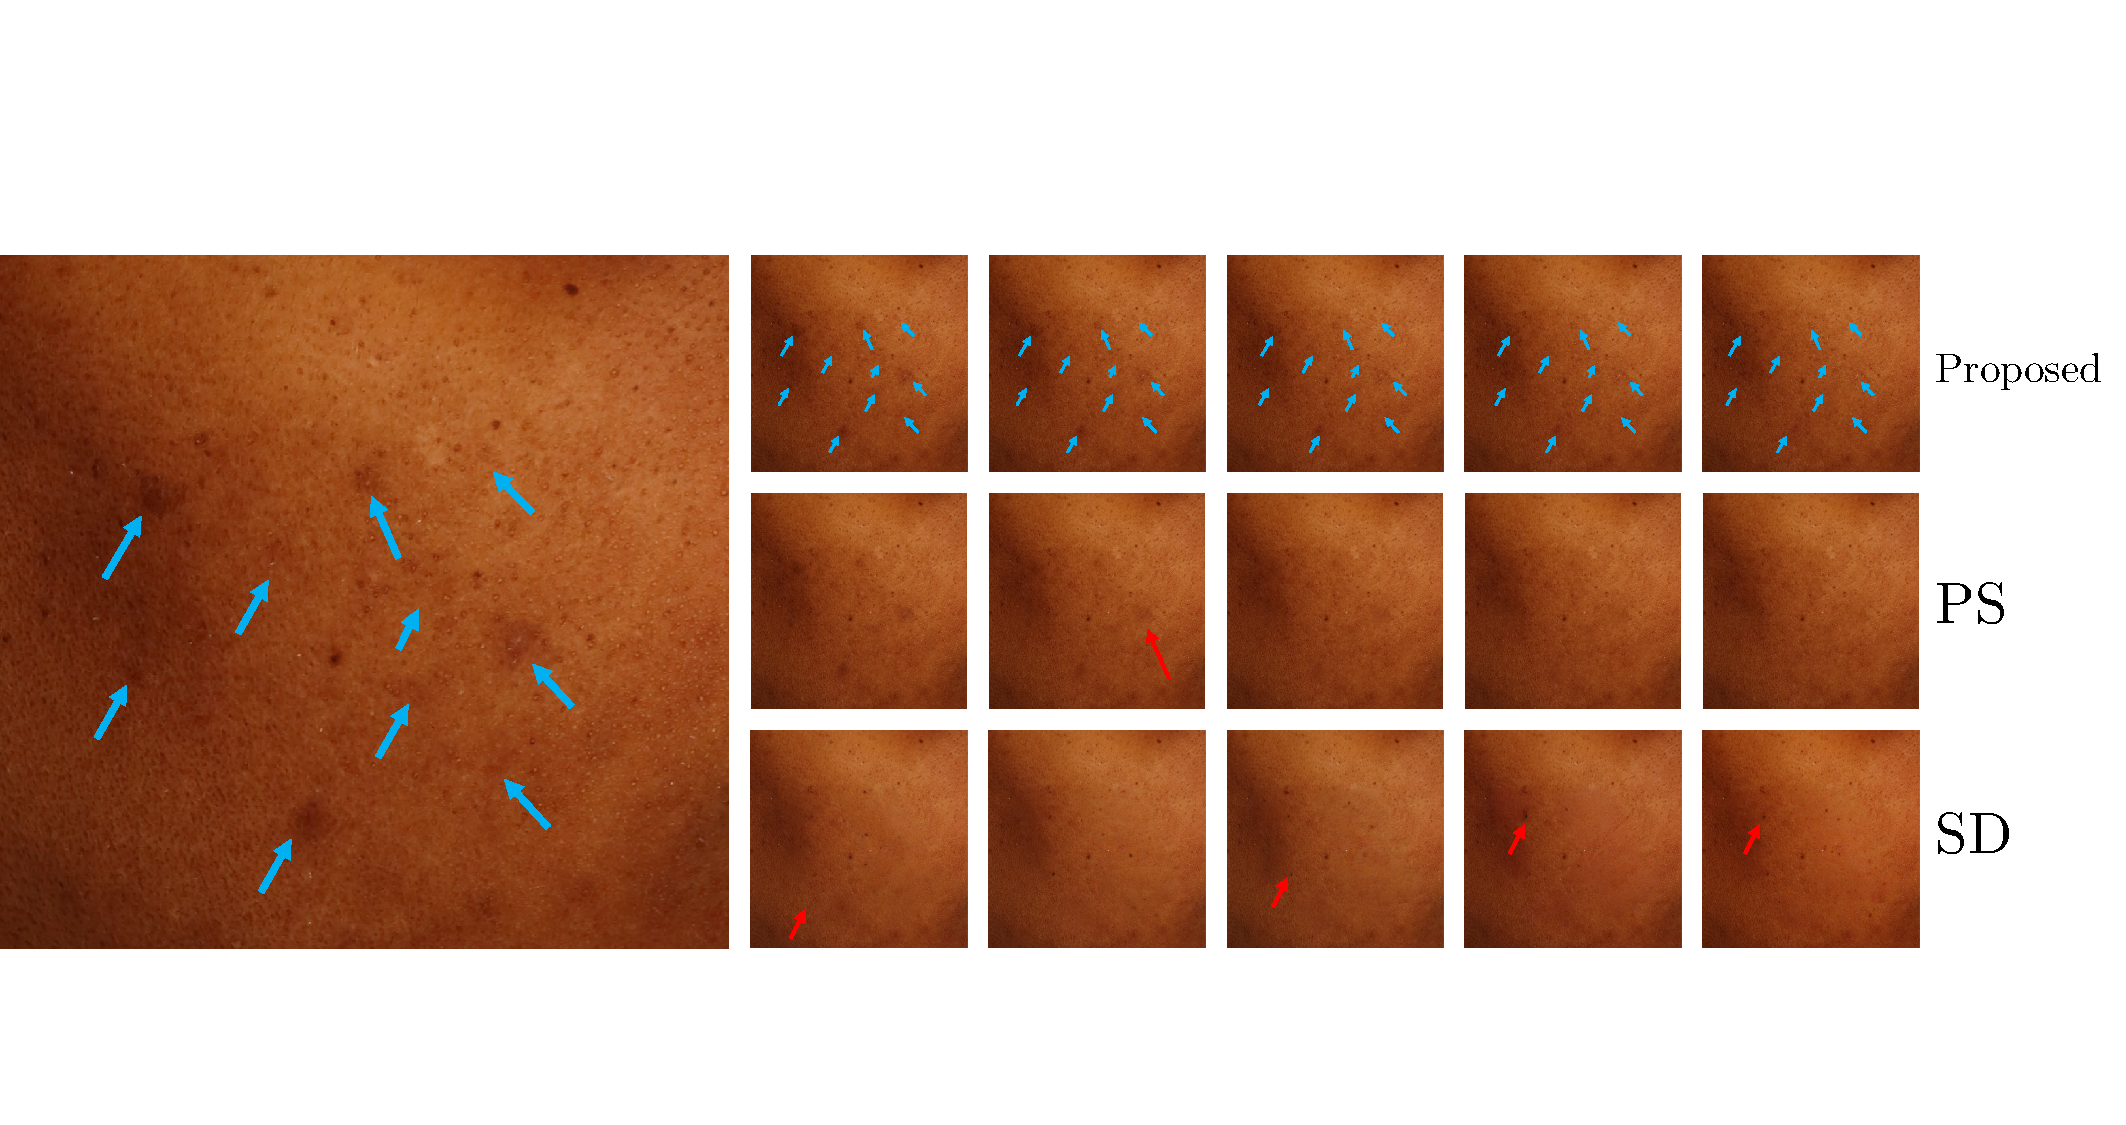
\includegraphics[width=\linewidth]{Chapter5/baseline/baseline43.pdf}
    \end{subfigure}
    \hfill
    \begin{subfigure}{\textwidth}
        \centering
        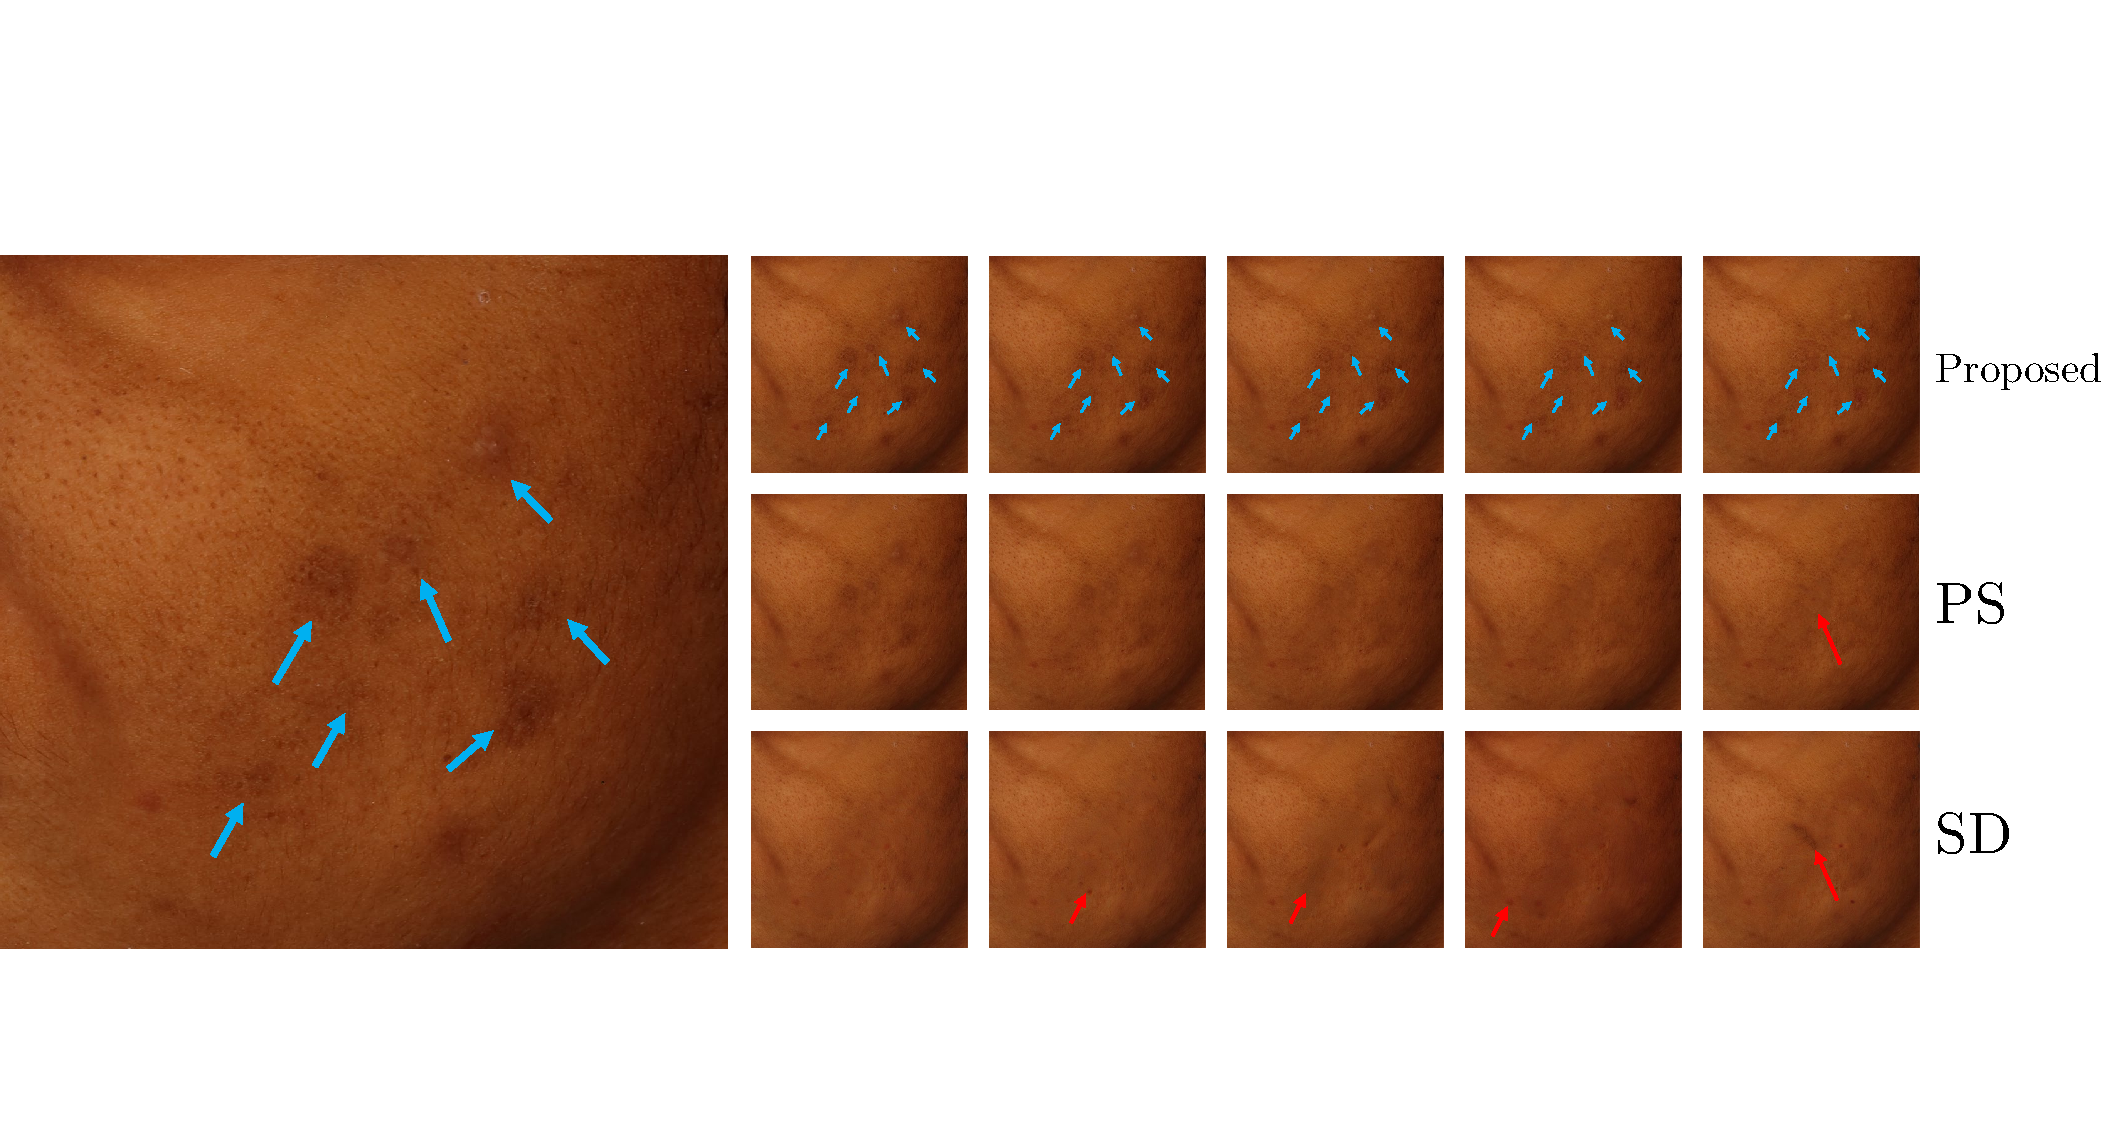
\includegraphics[width=\linewidth]{Chapter5/baseline/baseline44.pdf}
    \end{subfigure}
    \caption{Comparison with baseline methods. The results of several blemish removal or modification methods are compared, including the proposed method in question (marked as Ours), Adobe Photoshop\cite{adobephotoshop} inpainting (marked as PS), and Stable Diffusion\cite{rombach2021highresolution} inpainting (marked as SD). Arrows are manually added to highlight areas of interest. Note the red arrows where the PS produces over-smoothed skin patches and the SD produces visible artifacts. For darker skin tones, the SD method fails to simulate varying intermediate states of blemish removal, displaying similar results under different control intensities.}
    \label{fig:baseline}
\end{figure}

\begin{table}[t!]
    \caption{FID scores of different blemish fading rates. Lower scores are better.}
    \resizebox{\columnwidth}{!}{%
        \begin{tabular}{cccccc}
            \hline
            \multirow{2}{*}{Methods} & \multicolumn{5}{c}{Fading Rate}                                                                         \\ \cline{2-6}
                                     & 100\%                           & 80\%            & 60\%            & 40\%            & 20\%            \\ \hline\hline
            SD                       & 144.89                          & 133.53          & 134.16          & 160.10          & 159.54          \\
            PS                       & 117.98                          & 120.37          & 125.15          & 129.26          & \textbf{129.96} \\
            \textbf{Proposed}            & \textbf{115.30}                 & \textbf{118.12} & \textbf{122.64} & \textbf{127.09} & 131.60          \\ \hline
        \end{tabular}%
    }
    \label{tbl:fid}
\end{table}
\begin{figure}[t!]
    \centering
    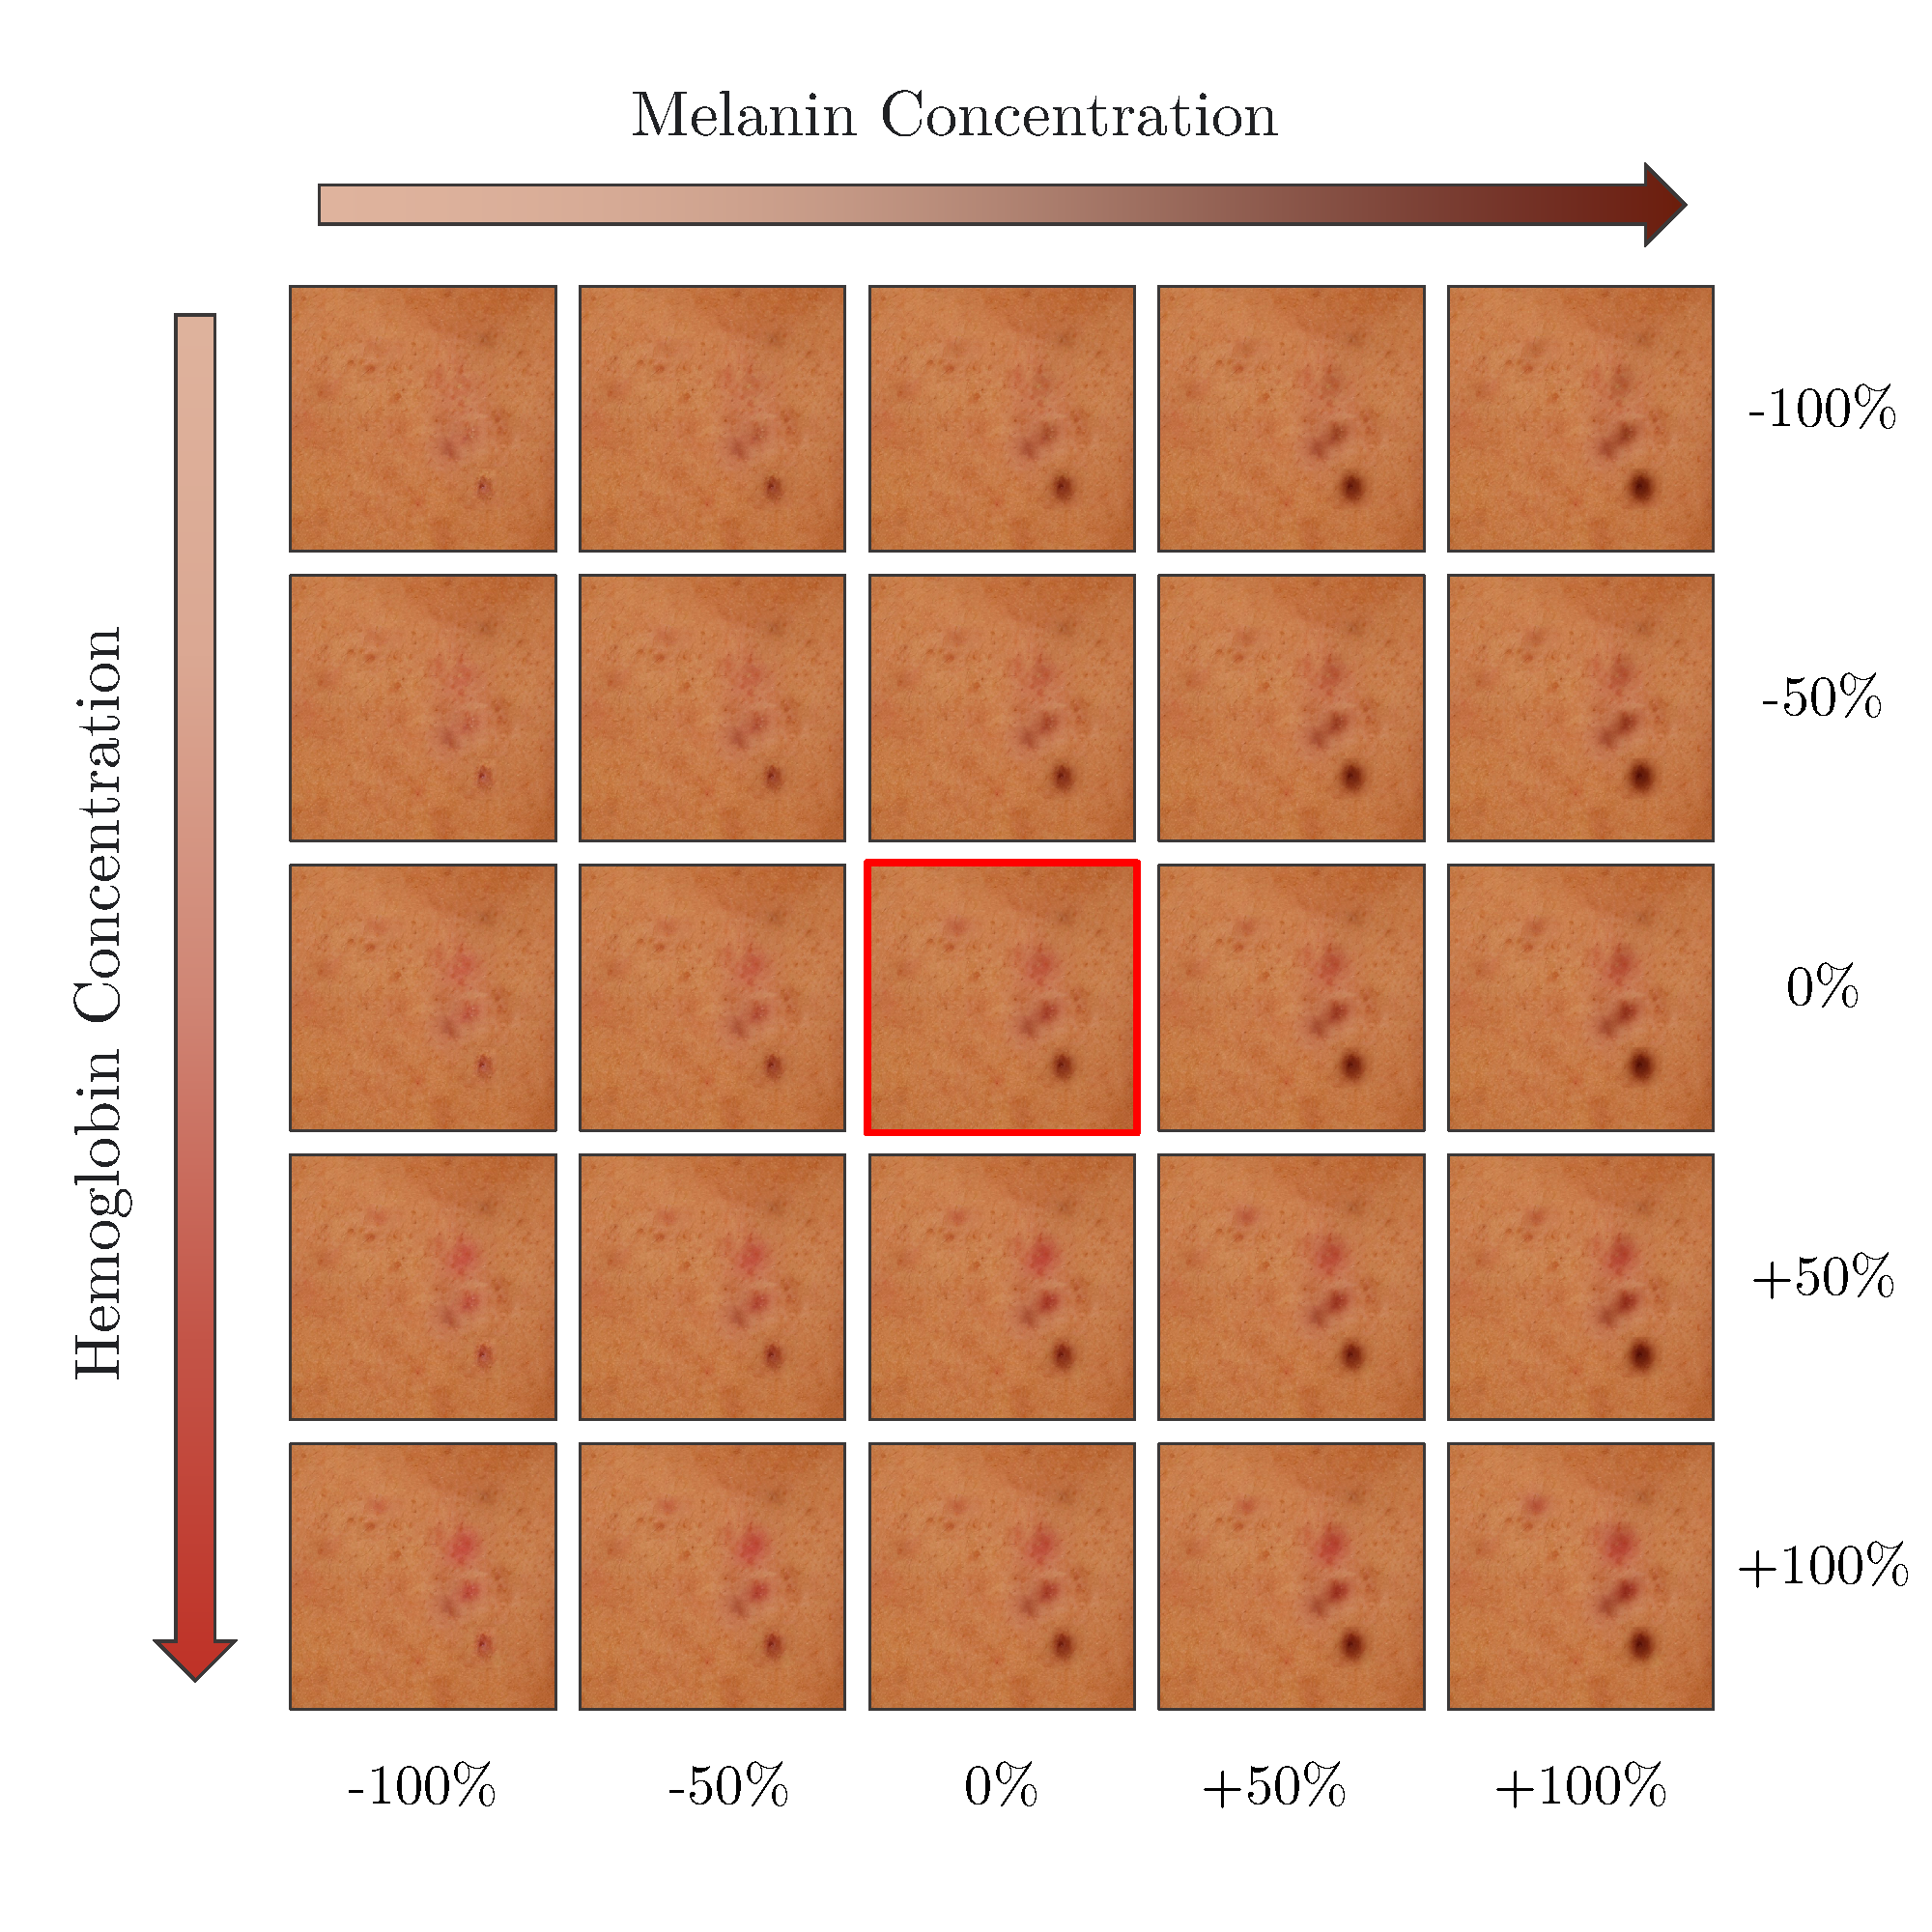
\includegraphics[width=0.96\columnwidth]{Chapter5/grid.pdf}
    \caption{Matrix of different chromophore concentrations setting. The original image is marked by a red box. The proposed model fully decouples the major chromophores of human skin, enabling highly controllable pigmentation editing.}
    \label{fig:matrix}
\end{figure}
For the FID scores, the proposed method achieved the lowest scores in the vast majority of cases, except for the 20\% fading rate. In particular, the proposed method has less variation in FID scores compared to other baselines at different fading rates, which suggests that the proposed model is able to achieve robust, realistic skin blemish simulations.

Visual comparison more intuitively demonstrates the superiority of the proposed algorithm. The PS method, although straightforward, led to a loss of skin detail through simple interpolation, resulting in blurry patches. Conversely, the SD method generated some contextually coherent skin details while removing the blemishes, but its quality was limited. Specifically, at higher denoising ratios, the SD method produced noticeable artifacts, and the modified areas differed in color from the surrounding skin.

The proposed method not only closely aligns with the natural degradation process of real skin but also ensures that the modified pigmentations match the underlying skin seamlessly. Unlike other techniques, this approach does not create artifacts or blurriness. It maintains skin details, including subtle textures such as hair and pores, leading to a natural appearance. This underlines the effectiveness of the proposed method in preserving the intricacy of skin texture while accomplishing realistic modifications.
\section{Controllability}
Controllability is key to user interaction with the proposed algorithm. A significant advantage of the proposed model is its high controllability, where users can freely adjust the parameters of the pigmentation to precisely control its appearance.
A changing matrix is plotted by adjusting the concentration control parameters of melanin and heamoglobin, as shown in Figure \ref{fig:matrix}. The proposed method successfully decouples the concentrations of these two chromophores, allowing users to independently control their apparent features, thus flexibly simulating the change of blemishes under different conditions.
\section{Perception Study}
\begin{figure}[t!]
    \centering
    \begin{subfigure}{.95\textwidth}
        \centering
        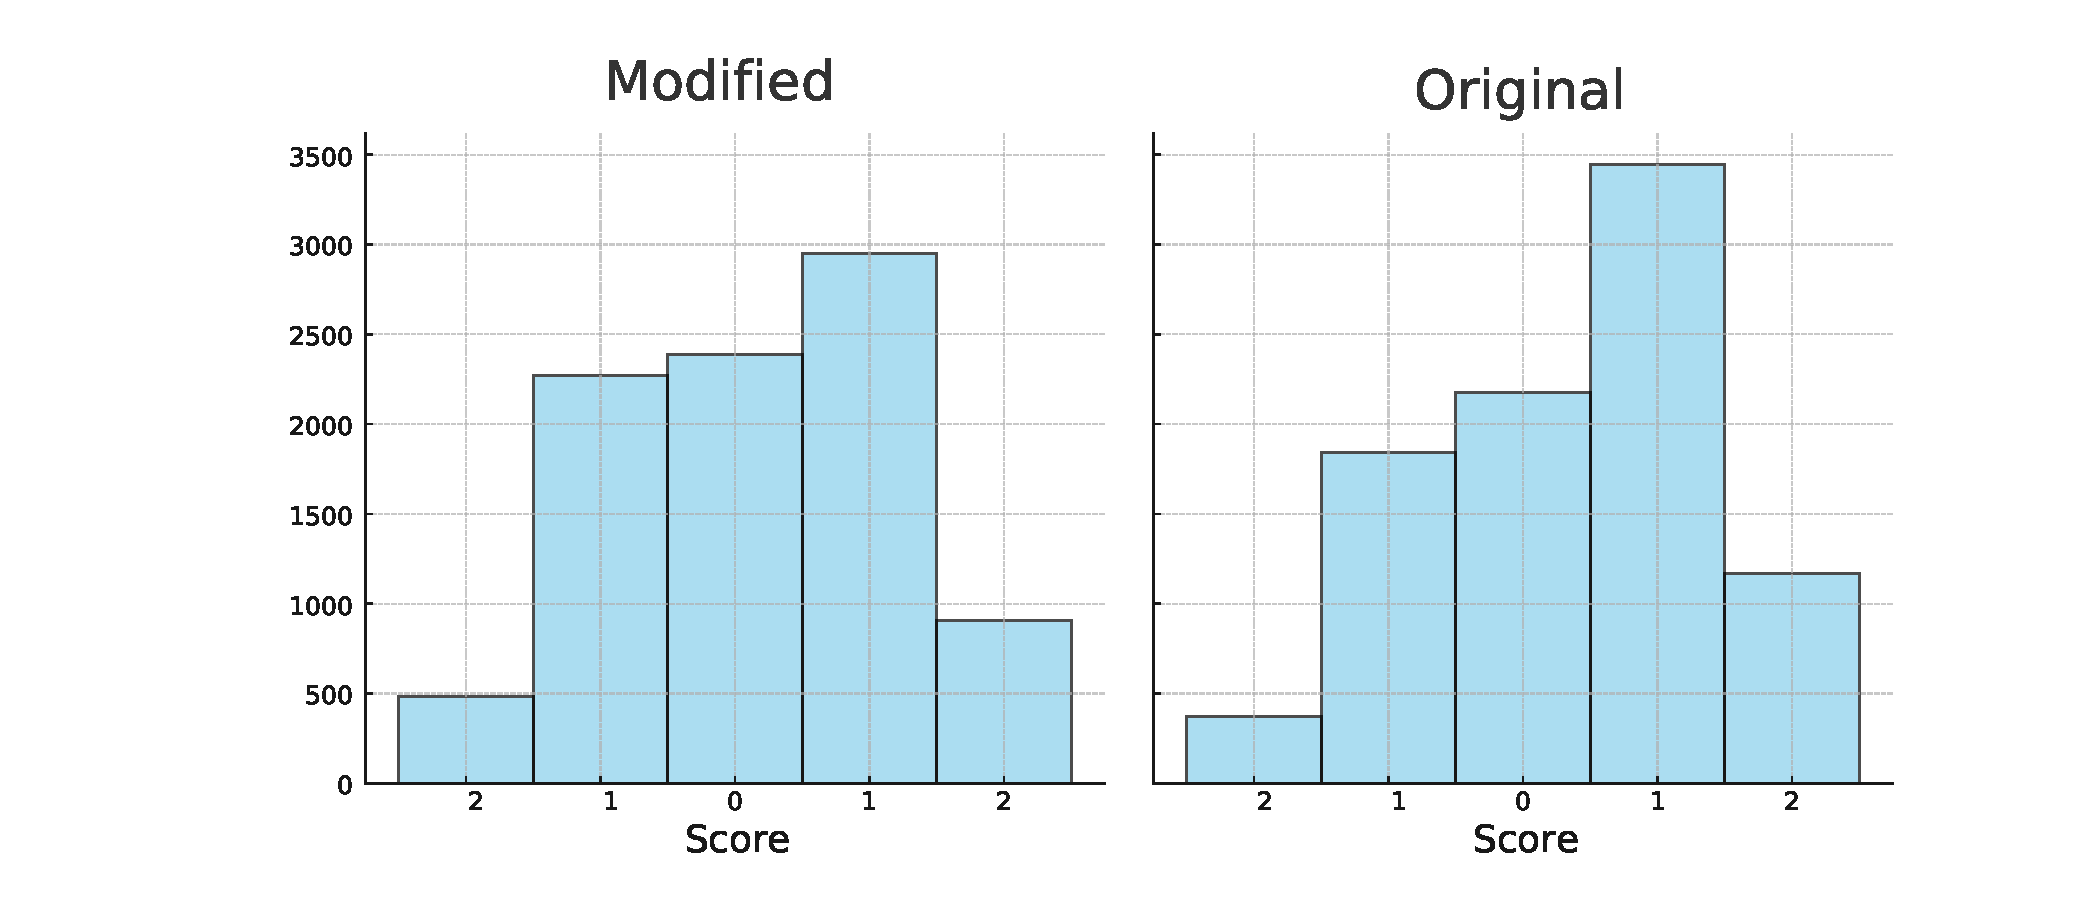
\includegraphics[width=0.95\columnwidth]{Chapter5/score.pdf}
        \caption{Scoring frequencies of survey responses}
        \label{fig:survey_hist}
    \end{subfigure}\hfill
    \begin{subfigure}{.95\textwidth}
        \centering
        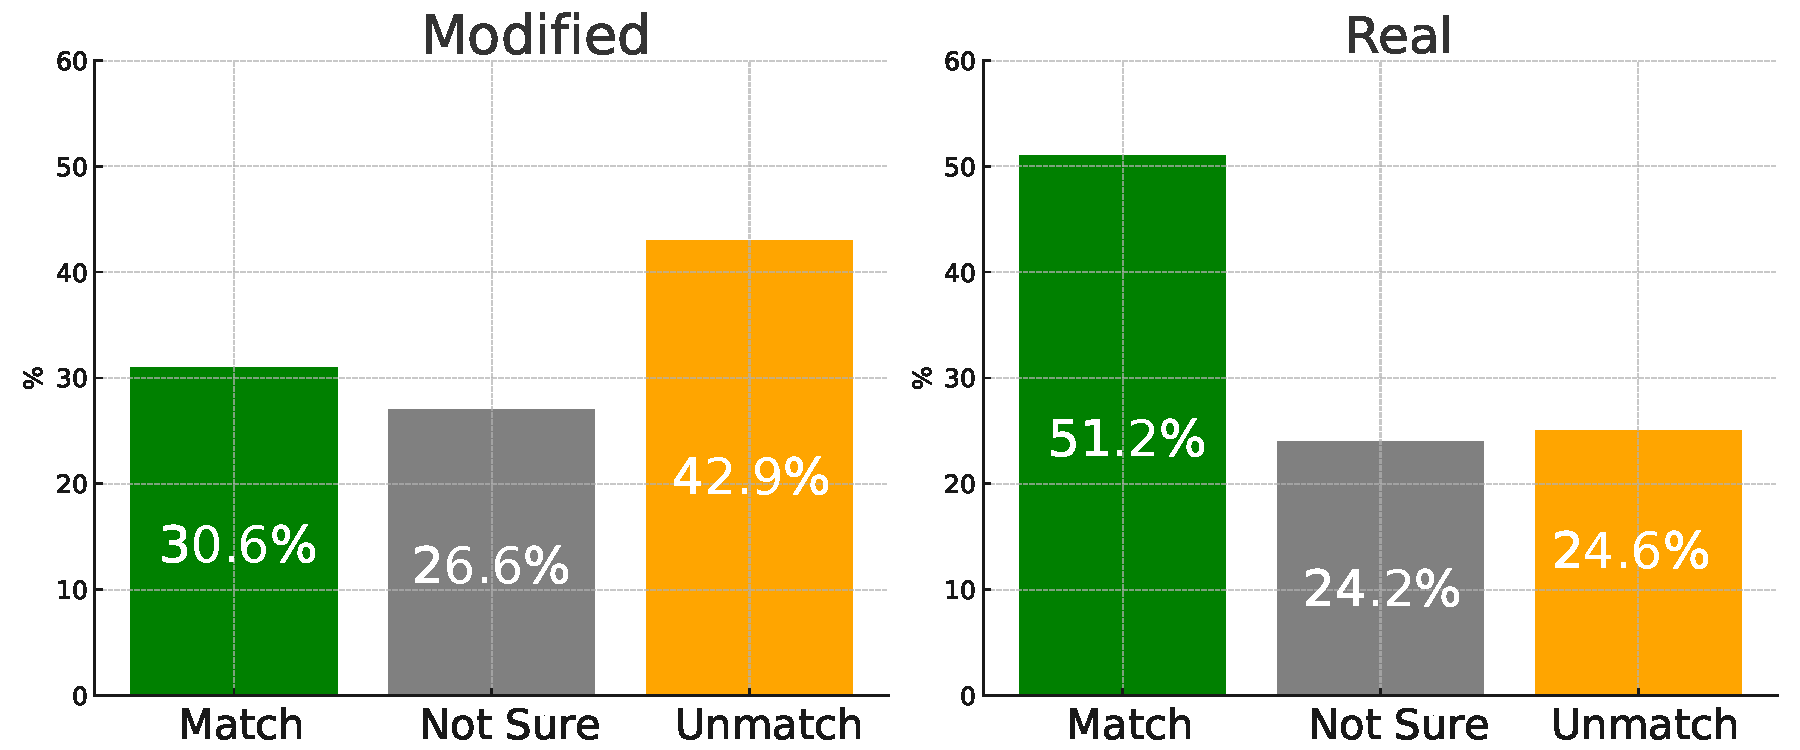
\includegraphics[width=0.95\columnwidth]{Chapter5/bar_charts_modified.pdf}
        \caption{Bar chart of survey results}
        \label{fig:bar_charts}
    \end{subfigure}
    \caption{Panellists scored images from -2 to +2 to assess their confidence in considering the image as modified or not, with higher scores indicating that the user considered the image to be unmodified. Scoring frequencies are displayed in Figure \ref{fig:survey_hist}. The results of the survey are shown in Figure \ref{fig:bar_charts}. For the modified images, more people perceived them as unmodified or not sure. This suggests that the modifications are consistent with human perception and intuition.}
\end{figure}
\begin{table}[t!]
    \caption{Key Statistics and Score Distribution from the Image Perception Study}
    \resizebox{\columnwidth}{!}{%
        \begin{tabular}{lrr}
            \hline
            \multicolumn{1}{l}{Score} & \multicolumn{1}{r}{Real Images (\%)} & \multicolumn{1}{r}{Fake Images (\%)} \\ \hline\hline
            -2 (Definitely Fake)      & 4.11  & 5.37  \\
            -1 (Likely Fake)          & 20.46 & 25.22 \\
            0 (Indistinguishable)     & 24.20 & \textbf{26.56} \\
            1 (Likely Real)           & 38.28 & 32.80 \\
            2 (Definitely Real)       & 12.96 & 10.06 \\ \hline
            \textbf{Average Score}    & 0.35511 & 0.16956 \\
            \textbf{Correctly Identified} & 51.23 & \textbf{30.59} \\
            \textbf{Failed to Identify (including Indistinguishable)} & 48.77 & \textbf{69.42} \\ \hline
        \end{tabular}%
    }
    \label{tbl:image_perception_stats}
\end{table}
The objective of this study is to evaluate if the pigmentation simulation is natural and believable. As shown in Figure \ref{fig:bar_charts} and Table \ref{tbl:image_perception_stats}, the altered images had a lower average score (0.16956 vs 0.35511), with only 30.6\% correctly identifying the altered image vs 23.6\% judging the real images as altered, and 26.6\% not sure if it is or is not altered. This indicates that the effect of the proposed algorithm is superior, to the point where laypeople cannot readily discern traces of algorithmic alteration.
The analysis revealed several key insights:
\begin{itemize}
    \item \textbf{Score Distribution} The distribution of scores for both real and altered images showed a significant overlap, especially for scores 0 and 1, indicating a level of ambiguity in distinguishing between real and simulated images.
    \item \textbf{Accuracy in Identification} Panellists correctly identified real images as real 51.23\% of the time, whereas they correctly identified altered images only 30.59\% of the time. This suggests a higher degree of realism in the simulated images.
    \item \textbf{Perception of Altered Images} Interestingly, a significant portion (42.86\%) of the altered images were perceived as real, and when considering scores of 0 as indistinguishable, this figure rose to 69.41\%. This underscores the effectiveness of the simulation in creating convincing images.
\end{itemize}
%=== END OF CHAPTER FIVE ===
\end{spacing}
\newpage
